% ==========================================
% BAB V IMPLEMENTASI
% ==========================================
\cleardoublepage
\chapter{IMPLEMENTASI SISTEM \textit{SMART WASTE BIN}}
\label{chap:implementasi}

Bab ini merupakan bagian kedua dari realisasi tahap \textit{Prototype} dalam metodologi \textit{Design Thinking}. Berdasarkan rancangan pada Bab IV, bab ini menjelaskan implementasi aktual setiap komponen sistem \textit{Smart Waste Bin}, mencakup peningkatan \textit{firmware} perangkat IoT, konfigurasi \textit{middleware} Node-RED, pembuatan \textit{database} Supabase, dan pengembangan \textit{dashboard} Next.js. Setiap subbab menjelaskan teknologi dan \textit{tools} yang digunakan, langkah-langkah implementasi, serta hasil yang diperoleh.

% ============================================================
\section{Implementasi Peningkatan \textit{Firmware}}
\label{sec:impl-firmware}
% ============================================================

Implementasi peningkatan \textit{firmware} dilakukan pada perangkat \textit{Smart Waste Bin} menggunakan Arduino IDE dengan \textit{board package} ESP32. Lima peningkatan yang dirancang pada Subbab \ref{sec:perancangan-firmware} diimplementasikan secara bertahap dan diuji sebelum di-\textit{deploy} ke perangkat di lapangan.

\subsection{Implementasi Perubahan Interval Pengambilan Data}

Interval \textit{deep sleep} diubah dari 8 jam menjadi 2 jam 30 menit dengan mendefinisikan konstanta waktu tidur dalam satuan mikrodetik, sebagaimana ditunjukkan pada \textit{Listing} \ref{lst:interval}.

\begin{lstlisting}[caption={Implementasi Perubahan Interval Pengambilan Data}, label={lst:interval}, language=C++]
// ===== SLEEP CONFIG =====
// 2.5 jam = 150 menit
uint64_t TIME_TO_SLEEP = 150ULL * 60ULL * 1000000ULL;
\end{lstlisting}

Perubahan interval ini menghasilkan 8--9 titik data per hari per perangkat, meningkat signifikan dari sebelumnya yang hanya 3 titik data per hari dengan interval 8 jam.

\subsection{Implementasi \textit{Median Filter}}

Pembacaan sensor diubah dari \textit{single reading} menjadi 5 kali pembacaan dengan pengambilan nilai median menggunakan algoritma \textit{bubble sort}, sebagaimana ditunjukkan pada \textit{Listing} \ref{lst:median}.

\begin{lstlisting}[caption={Implementasi \textit{Median Filter} pada Pembacaan Sensor}, label={lst:median}, language=C++]
const int numReadings = 5;
int readings[numReadings];
int validCount = 0;

for (int i = 0; i < numReadings; i++) {
    int reading = sensor.readRangeContinuousMillimeters();
    if (!sensor.timeoutOccurred() && reading > 0 && reading <= 1400) {
        readings[validCount] = reading;
        validCount++;
    }
    delay(100);
}

// Bubble sort for median
for (int i = 0; i < validCount - 1; i++) {
    for (int j = i + 1; j < validCount; j++) {
        if (readings[i] > readings[j]) {
            int temp = readings[i];
            readings[i] = readings[j];
            readings[j] = temp;
        }
    }
}

if (validCount >= 3) {
    a = readings[validCount / 2]; // Get median
} else if (validCount > 0) {
    int sum = 0;
    for (int i = 0; i < validCount; i++) sum += readings[i];
    a = sum / validCount;  // Fallback: mean
}
\end{lstlisting}

Implementasi ini mengurangi \textit{noise} pada data sensor. Nilai median dari 5 pembacaan mencegah pembacaan \textit{outlier} tunggal mempengaruhi hasil akhir, khususnya mencegah lompatan 10\% pada \textit{fillLevel} akibat \textit{truncation integer} dari perbedaan 1 unit \textit{raw}.

\subsection{Implementasi Mekanisme \textit{Auto-recovery}}

Mekanisme \textit{auto-recovery} diimplementasikan untuk menangani kondisi \textit{hang} pada sensor VL53L0X, sebagaimana ditunjukkan pada \textit{Listing} \ref{lst:recovery} dan \textit{Listing} \ref{lst:powercycle}.

\begin{lstlisting}[caption={Implementasi \textit{Auto-recovery} Sensor}, label={lst:recovery}, language=C++]
// Auto-recovery if sensor hangs (>= 3 timeout dari 5 pembacaan)
if (timeoutCount >= 3 || validCount == 0) {
    sensor.stopContinuous();
    delay(100);

    // Try soft reset first
    if (sensor.init(true)) {
        sensor.setMeasurementTimingBudget(200000);
        sensor.startContinuous(200);
        return; // Soft reset OK
    }

    // Soft reset failed, power cycle
    powerCycleSensor();
    if (!sensor.init(true)) {
        readSensor = false; // Sensor offline
    }
}
\end{lstlisting}

\begin{lstlisting}[caption={Implementasi \textit{Power Cycle} Sensor}, label={lst:powercycle}, language=C++]
void powerCycleSensor() {
    digitalWrite(TRIG_SENSOR, LOW);  // Turn off sensor power
    delay(500);                       // Wait for capacitor discharge
    digitalWrite(TRIG_SENSOR, HIGH); // Turn on again
    delay(300);                       // Wait for sensor boot
    Wire.end();
    delay(50);
    Wire.begin();                     // Re-init I2C
}
\end{lstlisting}

Mekanisme ini berhasil mencegah \textit{data loss} akibat sensor \textit{hang} yang sebelumnya memerlukan \textit{reset} manual.

\subsection{Implementasi \textit{Warm-up} Sensor}

Mekanisme \textit{warm-up} diimplementasikan sebagai bagian dari fungsi \texttt{initVL53L0X()} dengan 3 pembacaan \textit{dummy} setelah inisialisasi, sebagaimana ditunjukkan pada \textit{Listing} \ref{lst:warmup}.

\begin{lstlisting}[caption={Implementasi \textit{Warm-up} Sensor}, label={lst:warmup}, language=C++]
sensor.setMeasurementTimingBudget(200000);
delay(100);
sensor.startContinuous(200);

// Warm-up readings --- nilai dibuang, hanya untuk stabilisasi
SerialMon.println(F("Warming up sensor..."));
for (int i = 0; i < 3; i++) {
    sensor.readRangeContinuousMillimeters();
    delay(200);
}
SerialMon.println(F("Sensor ready!"));
\end{lstlisting}

Pendekatan ini memastikan pembacaan pertama data aktual sudah dalam kondisi sensor yang stabil, mengurangi risiko nilai anomali di awal setiap siklus pengukuran.

\subsection{Implementasi Optimasi Daya}

Optimasi daya diimplementasikan melalui \textit{GPIO isolation} sebelum \textit{deep sleep} untuk mencegah \textit{floating state}, sebagaimana ditunjukkan pada \textit{Listing} \ref{lst:gpio}.

\begin{lstlisting}[caption={Implementasi \textit{GPIO Isolation}}, label={lst:gpio}, language=C++]
// Turn off all GPIO
digitalWrite(TRIG, LOW);
digitalWrite(TRIG_SENSOR, LOW);
digitalWrite(LED_READ, LOW);
digitalWrite(LED_NET, LOW);

// Isolate GPIO (prevent floating during sleep)
gpio_hold_en(GPIO_NUM_13); // TRIG (modem power)
gpio_hold_en(GPIO_NUM_23); // TRIG_SENSOR
gpio_hold_en(GPIO_NUM_18); // LED_NET
gpio_hold_en(GPIO_NUM_19); // LED_READ
gpio_deep_sleep_hold_en();
\end{lstlisting}

% ============================================================
\section{Implementasi \textit{Middleware}}
\label{sec:impl-middleware}
% ============================================================

Berdasarkan rancangan \textit{flow} dan spesifikasi \textit{node} pada Subbab \ref{sec:perancangan-middleware}, \textit{middleware} diimplementasikan menggunakan Node-RED v4.1.3 yang berjalan pada \textit{server} lokal dengan Node.js v24.12.0. Berbeda dengan Bab \ref{chap:perancangan} yang membahas rancangan, subbab ini menyajikan realisasi konfigurasi aktual setiap \textit{node} beserta pengujian alur data menggunakan \textit{node} Inject.

Gambar \ref{fig:flow-nodered-impl} menunjukkan realisasi \textit{flow} Node-RED yang telah dibangun, mencakup \textit{node} MQTT In, JSON, HTTP Request, Debug, dan Inject untuk ketiga sensor.

\begin{figure}[H]
  \caption{Realisasi \textit{Flow} Node-RED pada Node-RED Editor}
  \label{fig:flow-nodered-impl}
  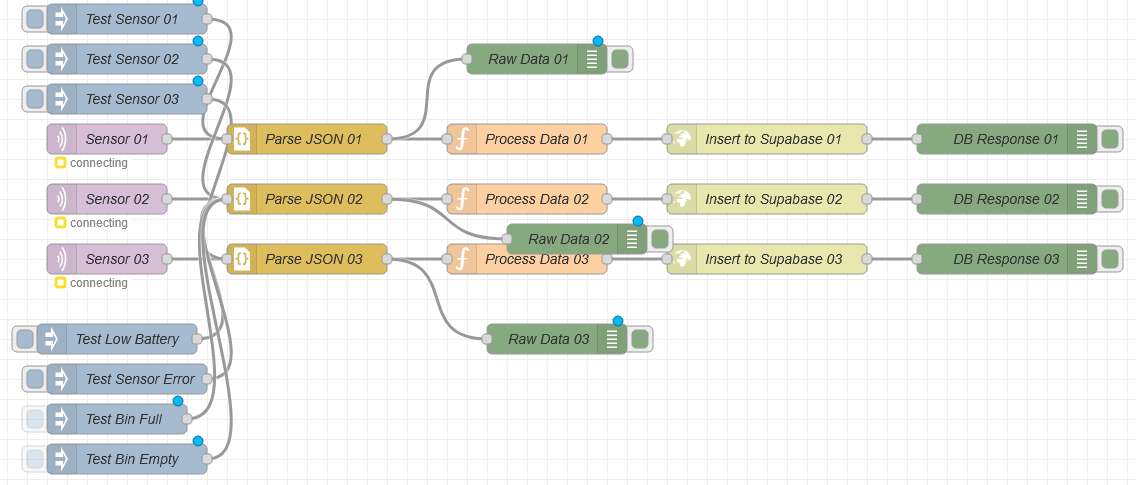
\includegraphics[width=\textwidth]{images/flow-nodered-impl.png}
  % RENAME: tangkapan layar (screenshot) flow Node-RED aktual dari Node-RED editor.
  %         Berbeda dengan Gambar di Bab IV yang berupa diagram alur generik (rancangan),
  %         gambar ini adalah realisasi nyata flow yang sudah dibangun.
\end{figure}

\subsection{Konfigurasi \textit{Node} MQTT In}

\textit{Node} MQTT In berfungsi sebagai \textit{subscriber} yang menerima data dari \textit{broker}. Tabel \ref{tab:konfigurasi-mqtt-node} menyajikan konfigurasi aktual yang digunakan.

\begin{table}[H]
  \caption{Konfigurasi \textit{Node} MQTT In}
  \label{tab:konfigurasi-mqtt-node}
  \begin{tabularx}{\textwidth}{| l | l | X |}
    \hline
    \textbf{Parameter} & \textbf{Nilai} & \textbf{Keterangan} \\
    \hline
    \textit{Server} & (IP \textit{Broker}) & Alamat MQTT \textit{broker} \\
    \hline
    Port & 1883 & Port default MQTT \\
    \hline
    \textit{Topic} & \texttt{wp2/basic\_01}, \texttt{wp2/basic\_02}, \texttt{wp2/basic\_03} & Satu \textit{topic} per sensor \\
    \hline
    \textit{Output} & Auto-detect & Otomatis deteksi tipe data \\
    \hline
  \end{tabularx}
\end{table}

\subsection{Konfigurasi \textit{Node} JSON}

\textit{Node} JSON mengkonversi \textit{payload} dari format string JSON menjadi objek JavaScript yang dapat diproses lebih lanjut. Tabel \ref{tab:impl-konfigurasi-json} menyajikan konfigurasi yang digunakan.

\begin{table}[H]
  \caption{Konfigurasi \textit{Node} JSON}
  \label{tab:impl-konfigurasi-json}
  \begin{tabularx}{\textwidth}{| l | l | X |}
    \hline
    \textbf{Parameter} & \textbf{Nilai} & \textbf{Keterangan} \\
    \hline
    Action & Convert between JSON String \& Object & Mengubah string ke objek \\
    \hline
    Property & msg.payload & Lokasi data yang dikonversi \\
    \hline
    Format JSON String & Tidak dicentang & \textit{Output} berupa objek, bukan string \\
    \hline
  \end{tabularx}
\end{table}

\subsection{Konfigurasi \textit{Node} HTTP Request}

\textit{Node} HTTP Request mengirimkan data ke \textit{database} Supabase menggunakan REST API. Tabel \ref{tab:konfigurasi-http} menyajikan parameter konfigurasinya, dan Tabel \ref{tab:konfigurasi-headers} menyajikan \textit{header} autentikasi yang digunakan.

\begin{table}[H]
  \caption{Konfigurasi \textit{Node} HTTP Request}
  \label{tab:konfigurasi-http}
  \begin{tabularx}{\textwidth}{| l | X |}
    \hline
    \textbf{Parameter} & \textbf{Nilai} \\
    \hline
    Method & POST \\
    \hline
    URL & \texttt{https://[project-ref]\allowbreak.supabase.co\allowbreak/rest\allowbreak/v1\allowbreak/sensor\_data} \\
    \hline
    \textit{Payload} & Dikirim sebagai \textit{request body} \\
    \hline
    Return & UTF-8 String \\
    \hline
  \end{tabularx}
\end{table}

\begin{table}[H]
  \caption{Konfigurasi HTTP \textit{Headers}}
  \label{tab:konfigurasi-headers}
  \begin{tabularx}{\textwidth}{| l | l | X |}
    \hline
    \textbf{\textit{Header}} & \textbf{Nilai} & \textbf{Keterangan} \\
    \hline
    \texttt{apikey} & [Supabase anon key] & API key untuk autentikasi \\
    \hline
    \texttt{Authorization} & Bearer [anon key] & Token autentikasi \\
    \hline
    \texttt{Content-Type} & application/json & Format data yang dikirim \\
    \hline
    \texttt{Prefer} & return=representation & Mengembalikan data yang berhasil disimpan \\
    \hline
  \end{tabularx}
\end{table}

\subsection{Konfigurasi \textit{Node} Debug}

\textit{Node} Debug menampilkan data pada \textit{sidebar} Node-RED untuk keperluan \textit{monitoring} dan \textit{debugging}. Tabel \ref{tab:impl-konfigurasi-debug} menyajikan konfigurasi yang digunakan.

\begin{table}[H]
  \caption{Konfigurasi \textit{Node} Debug}
  \label{tab:impl-konfigurasi-debug}
  \begin{tabularx}{\textwidth}{| l | l | X |}
    \hline
    \textbf{Nama \textit{Node}} & \textbf{\textit{Output}} & \textbf{Fungsi} \\
    \hline
    \textit{Raw data} 01/02/03 & msg.payload & Menampilkan data mentah setelah \textit{parsing} JSON \\
    \hline
    Authorization & msg.payload & Menampilkan \textit{response} dari Supabase \\
    \hline
  \end{tabularx}
\end{table}

\subsection{Konfigurasi \textit{Node} Inject}

\textit{Node} Inject digunakan untuk pengujian \textit{flow} tanpa menunggu data dari perangkat IoT. Tabel \ref{tab:impl-konfigurasi-inject} menyajikan daftar skenario pengujian yang diimplementasikan.

\begin{table}[H]
  \caption{Konfigurasi \textit{Node} Inject untuk Pengujian}
  \label{tab:impl-konfigurasi-inject}
  \begin{tabularx}{\textwidth}{| l | X | X |}
    \hline
    \textbf{Nama \textit{Node}} & \textbf{Skenario} & \textbf{Karakteristik Data} \\
    \hline
    Test Sensor 01/02/03 & Data normal per sensor & Semua nilai dalam rentang normal \\
    \hline
    Test Low \textit{Battery} & Baterai rendah & \texttt{battPercent} $<$ 30\%, \textit{event}: ``LowBattery'' \\
    \hline
    Test Sensor Error & Sensor tidak tersedia & Nilai 999, \texttt{ina219\_avail}: false \\
    \hline
    Test Bin Full & Tempat sampah penuh & \texttt{fillLevel}: 100, \texttt{dist}: 0 \\
    \hline
    Test Bin Empty & Tempat sampah kosong & \texttt{fillLevel}: 0, \texttt{dist}: tinggi \\
    \hline
  \end{tabularx}
\end{table}

\subsection{Alur Pemrosesan Data}

Berdasarkan konfigurasi \textit{node} yang telah dijelaskan, alur pemrosesan data pada \textit{middleware} adalah sebagai berikut. Pertama, \textit{node} MQTT In menerima pesan dari \textit{broker} dengan QoS \textit{level} 0. Kedua, \textit{node} JSON mengkonversi string \textit{payload} menjadi objek JavaScript. Ketiga, \textit{node} Function melakukan \textit{mapping field} dan menambahkan metadata berupa \textit{timestamp server} dan \texttt{device\_topic}. Keempat, \textit{node} HTTP Request mengirimkan data ke Supabase via REST API. \textit{Response} dari \textit{database} ditampilkan pada \textit{node} Debug untuk \textit{monitoring}.

% ============================================================
\section{Implementasi \textit{Database}}
\label{sec:impl-database}
% ============================================================

\textit{Database} diimplementasikan menggunakan Supabase yang merupakan \textit{platform Backend-as-a-Service} berbasis PostgreSQL. Implementasi mencakup pembuatan tabel \texttt{sensor\_data} dan konfigurasi akses API.

Sistem menggunakan satu tabel utama bernama \texttt{sensor\_data} untuk menyimpan seluruh data pembacaan sensor. Desain ini dipilih karena data yang dikumpulkan bersifat \textit{time-series} dengan struktur seragam dari semua perangkat. Gambar \ref{fig:tabel-sensordata} menunjukkan struktur tabel \texttt{sensor\_data} pada Supabase, dan Tabel \ref{tab:impl-detail-sensordata} menjelaskan spesifikasi setiap kolom.

\begin{table}[H]
  \caption{Detail Kolom Tabel \texttt{sensor\_data}}
  \label{tab:impl-detail-sensordata}
  \begin{tabularx}{\textwidth}{| l | l | l | X |}
    \hline
    \textbf{Kolom} & \textbf{Tipe Data} & \textbf{\textit{Constraint}} & \textbf{Deskripsi} \\
    \hline
    \texttt{id} & int8 & PK, Auto-increment & Identifier unik \textit{record} \\
    \hline
    \texttt{sensor\_id} & text & Not Null & Identifier perangkat sensor \\
    \hline
    \texttt{tegangan} & Numeric & Nullable & Tegangan baterai (Volt) \\
    \hline
    \texttt{arus} & Numeric & Nullable & Arus baterai (mA) \\
    \hline
    \texttt{daya} & Numeric & Nullable & Daya terpakai (mW) \\
    \hline
    \texttt{batt\_percent} & Numeric & Nullable & Persentase baterai (\%) \\
    \hline
    \texttt{ina219\_avail} & Bool & Nullable & Status ketersediaan sensor INA219 \\
    \hline
    \texttt{fillLevel} & Int4 & Nullable & Tingkat kepenuhan (0--100\%) \\
    \hline
    \texttt{distance} & Int4 & Nullable & Jarak terukur (mm) \\
    \hline
    \texttt{volume} & Int4 & Nullable & Volume sampah (dm³) \\
    \hline
    \texttt{vl53l0x\_avail} & Int4 & Nullable & Ketersediaan sensor VL53L0X (1/0) \\
    \hline
    \texttt{event} & text & Nullable & Tipe \textit{event} (DataUpdate, LowBattery, dll.) \\
    \hline
    \texttt{device\_topic} & text & Nullable & \textit{Topic} MQTT sumber data \\
    \hline
    \texttt{timestamp} & timestamptz & Nullable & Waktu pembacaan sensor (dari perangkat) \\
    \hline
    \texttt{created\_at} & timestamptz & Nullable & Waktu data disimpan di \textit{database} \\
    \hline
  \end{tabularx}
\end{table}

\textit{Field} \texttt{timestamp} mencatat waktu pembacaan di perangkat IoT, sedangkan \texttt{created\_at} mencatat waktu data diterima dan disimpan di \textit{database}. Selisih antara keduanya menunjukkan latensi transmisi data dari perangkat ke \textit{database}.

% ============================================================
\section{Implementasi \textit{Dashboard}}
\label{sec:impl-dashboard}
% ============================================================

\textit{Dashboard} diimplementasikan menggunakan Next.js sebagai \textit{framework} utama dan di-\textit{deploy} pada \textit{platform} Vercel. Subbab ini menjelaskan implementasi API, antarmuka pengguna, dan \textit{hosting}.

\subsection{Implementasi API}

\textit{Dashboard} berkomunikasi dengan \textit{database} melalui API Routes yang disediakan Next.js. \textit{Endpoint} \texttt{/api\allowbreak/sensor-data} diimplementasikan pada file \texttt{src\allowbreak/app\allowbreak/api\allowbreak/sensor-data\allowbreak/route.ts} dan mendukung operasi CRUD untuk manajemen data sensor. Gambar \ref{fig:api-response} menunjukkan contoh \textit{response} dari API GET.

\begin{figure}[H]
  \caption{Contoh \textit{Response} API GET}
  \label{fig:api-response}
  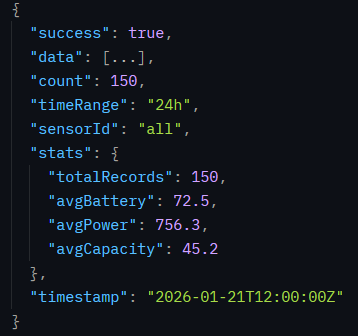
\includegraphics[width=0.65\textwidth]{images/api-response.png}
  % RENAME: image14.png → api-response.png
\end{figure}

\textit{Response} API mencakup data sensor, jumlah \textit{record}, serta statistik agregat yang dihitung langsung di \textit{database} menggunakan fungsi SQL \texttt{AVG()} dan \texttt{COUNT()}.

\subsection{Implementasi Antarmuka}

Antarmuka \textit{dashboard} diimplementasikan sebagai komponen React pada file \texttt{src\allowbreak/components\allowbreak/Dashboard.tsx}. Komponen ini menggunakan React Hooks untuk manajemen \textit{state} dan \textit{side effects}. Tabel \ref{tab:state-variable} menyajikan \textit{state variable} yang digunakan.

\begin{table}[H]
  \caption{\textit{State Variable} Komponen \textit{Dashboard}}
  \label{tab:state-variable}
  \begin{tabularx}{\textwidth}{| l | l | X |}
    \hline
    \textbf{\textit{State Variable}} & \textbf{Tipe} & \textbf{Deskripsi} \\
    \hline
    \texttt{selectedSensor} & string & Menyimpan ID sensor yang dipilih atau ``all'' untuk semua sensor \\
    \hline
    \texttt{timerange} & string & Rentang waktu data yang ditampilkan (24h, 7d, 30d) \\
    \hline
    \texttt{sensorData} & SensorDataPoint[] & \textit{Array} data mentah dari sensor yang diterima dari API \\
    \hline
    \texttt{processedData} & any[] & Data yang telah diproses untuk visualisasi \textit{chart} \\
    \hline
    \texttt{sensorStats} & object & Statistik agregat untuk setiap sensor \\
    \hline
    \texttt{loading} & boolean & Status \textit{loading} saat \textit{fetching} data \\
    \hline
    \texttt{lastUpdate} & Date \textbar{} null & \textit{Timestamp} pembaruan data terakhir \\
    \hline
    \texttt{availableSensors} & Number[] & Daftar sensor ID yang tersedia untuk opsi \textit{dropdown} \\
    \hline
  \end{tabularx}
\end{table}

\textit{Dashboard} terdiri dari enam komponen utama sebagai berikut.

\begin{enumerate}
  \item \textbf{\textit{Header Section}}: menampilkan judul aplikasi, tombol \textit{refresh} manual, dan informasi \textit{timestamp} pembaruan terakhir.

  \item \textbf{\textit{Sensor Status Cards}}: menampilkan kartu status untuk setiap sensor aktif, mencakup ID sensor, status operasional (NORMAL, WARNING, atau CRITICAL), \textit{fill level} dengan \textit{progress bar} berwarna (hijau $\leq$70\%, kuning 71--85\%, merah $>$85\%), persentase baterai, konsumsi daya, \textit{topic} MQTT, dan \textit{timestamp} terakhir.

  \item \textbf{\textit{Control Panel}}: menyediakan \textit{dropdown} pemilihan sensor, \textit{dropdown} rentang waktu (Last 24 Hours, Last 7 Days, Last 30 Days), serta informasi jumlah \textit{data points} dan \textit{active sensors}.

  \item \textbf{Visualisasi Data}: dua \textit{chart} interaktif menggunakan Recharts: \textit{Waste Fill Level Trend} (\textit{line chart} tren kepenuhan) dan \textit{Battery \& Power Consumption} (\textit{dual-axis line chart} baterai dan konsumsi daya).

  \item \textbf{\textit{Recent Sensor Readings}}: tabel 10 pembacaan sensor terbaru dengan \textit{progress bar} mini dan \textit{status indicator} berwarna.

  \item \textbf{\textit{System Analytics}}: lima metrik agregat: Total Records, Active Sensors, Avg Battery, Avg Power, dan Critical Alerts.
\end{enumerate}

\textit{Dashboard} mengimplementasikan \textit{auto-refresh} setiap 30 detik menggunakan \texttt{useEffect} Hook dengan \texttt{setInterval} dan \textit{cleanup function} untuk mencegah \textit{memory leak}. Tampilan lengkap antarmuka \textit{dashboard} disajikan pada Lampiran B.

\subsection{\textit{Deployment Dashboard}}

\textit{Dashboard} di-\textit{deploy} menggunakan \textit{platform} Vercel melalui integrasi Git. Setiap \textit{push} ke \textit{branch} utama memicu proses \textit{build} dan \textit{deployment} secara otomatis (\textit{Continuous Deployment}). Tabel \ref{tab:impl-hosting} menyajikan spesifikasi \textit{hosting} yang digunakan.

\begin{table}[H]
  \caption{Spesifikasi \textit{Hosting Dashboard}}
  \label{tab:impl-hosting}
  \begin{tabularx}{\textwidth}{| l | X |}
    \hline
    \textbf{Aspek} & \textbf{Spesifikasi} \\
    \hline
    \textit{Platform} & Vercel (\textit{free tier}) \\
    \hline
    \textit{Framework Preset} & Next.js \\
    \hline
    \textit{Build Command} & \texttt{next build} \\
    \hline
    \textit{Output Directory} & \texttt{.next} \\
    \hline
    \textit{Deployment Method} & Git Integration (\textit{Continuous Deployment}) \\
    \hline
    Domain & Subdomain Vercel (\texttt{*.vercel.app}) \\
    \hline
  \end{tabularx}
\end{table}